\chapter{Conclusion} % Main chapter title

\label{Chapitre4} % For referencing the chapter elsewhere, use \ref{Chapter1} 

\lhead{Chapitre 4. \emph{Conclusion}} % This is for the header on each page - perhaps a shortened title
Dans ce travail de recherche, nous avons étudier les variations par rapport aux prévisions dans la gestion des projets informatiques. Nous avions pour objectif d'étudier les variations et de proposer un modèle de gestion de ces variations pendant la gestion du projet.\\
Nous avons proposer deux solutions: une première solution basée sur les PSEE et une seconde solution avec un fichier excel.\\
La première solution est composée de trois parties: le méta-modèle pour décrire les procédés, la technique de détection des variations et le plan de correction pour la variation détectée.\\
La seconde solution a été mise en place suite à une discussion avec un chef de projet chez Alstom. C'est un macro excel permettant de détecter les variations grâce aux paramètres qu'on lui fournit et nous affiche les résultats sous forme de graphe. \\
Même si ces solutions permettent de détecter quelques variations, et aident le chef de projet dans la prise de décision; elles ne peuvent pas détecter tous les types de variations.\\
\textbf{Limites et perspectives}: les limites et les perspectives d'amélioration de nos deux solutions sont:\\
\textbf{Solution 1}:\\
Notre première solution est assez limité car elle ne permet pas d'anticiper la détection des variations. La variation n'est détectée que lorsque les tâches sont terminées.\\
\textbf{Solution 2}:\\
Les diagrammes résultant de l'exploitation de notre modèle de fichier Excel initialement mis en place et nous permettent à travers des représentations graphiques de voir systématiquement la variation sur les dates de début et de réalisation des tâches. \\
Par rapport aux diagrammes~\ref{graphe1} et~\ref{graphe2} on pourra améliorer ces derniers en traçant une droite horizontale qui représente la date de validité (date à laquelle les données ont été mises à jour), on aurait pu séparer les taches précédentes des tâches futures à venir~\ref{graphe4}.
\begin{figure}[h]
\centering
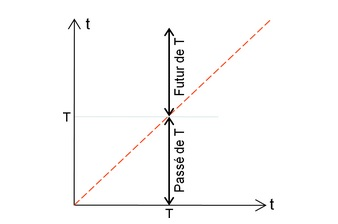
\includegraphics[width=9cm]{graphe4.jpg}
\caption{\label{graphe2}Amélioration}
\end{figure}
D'autres types d'indicateurs peuvent également être mis en  place en fonction des besoins. On pourra par exemple mettre en place un tableau de synthèse de variations qui pourra être importé dans un autre outil etc.
